\documentclass{beamer}

\usepackage{biblatex}
\bibliography{bibliography}
\AtBeginBibliography{\small}
\usepackage{hyperref}

\usetheme{Antibes}
\usecolortheme{beaver}

\title{Operatore di Koopman}
\subtitle{Identificazione dell'EKF}
\author{Sergio Vanegas}
\institute{Modelway S.r.l.}
\date{\today}

\begin{document}

\frame{\titlepage}

\begin{frame}{Struttura di riferimento}
    \begin{figure}
        \centering
        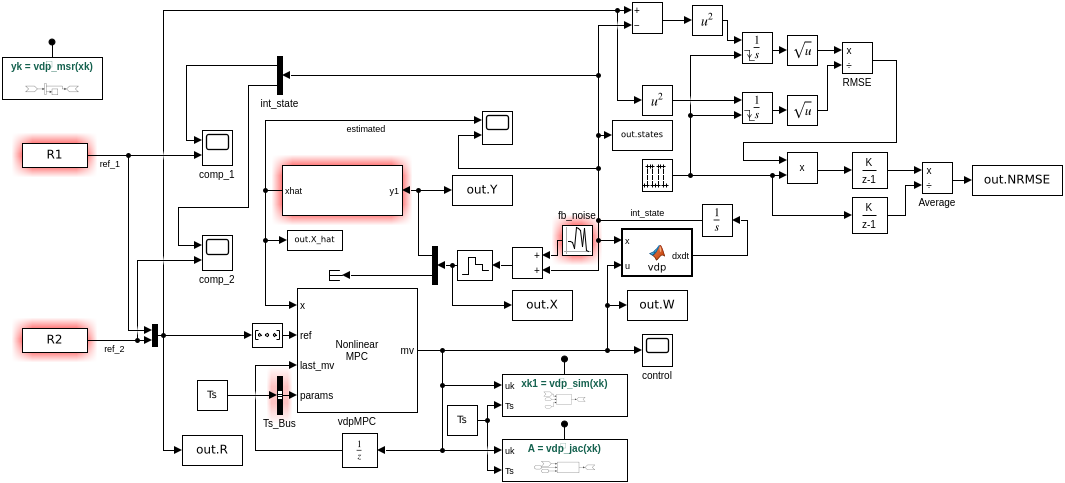
\includegraphics[width=\textwidth]{Figures/Kalman_nlMPC.png}
        \caption{Ciclo di controllo originale}
    \end{figure}
\end{frame}

\begin{frame}{Partizione dei segnali}
    \begin{itemize}
        \item Ingressi
        \begin{itemize}
            \item Uscita dell'oscillatore
            \item Ultimo segnale di controllo
        \end{itemize}
        \item Stati
        \begin{itemize}
            \item Stima degli stati
            \item Elementi della matrice di covarianza (ozionale)
        \end{itemize}
        \item Uscita: stima degli stati
    \end{itemize}
\end{frame}

\begin{frame}[allowframebreaks]{Sostituzione dell'EKF}
    \begin{figure}
        \centering
        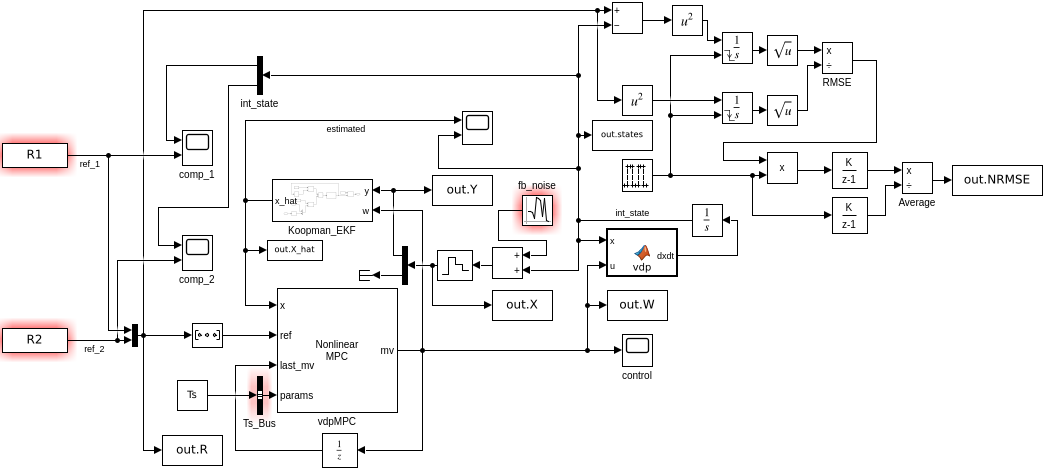
\includegraphics[width=\textwidth]{Figures/Koopman_nlMPC.png}
        \caption{Nuovo ciclo di controllo}
    \end{figure}

    \begin{figure}
        \centering
        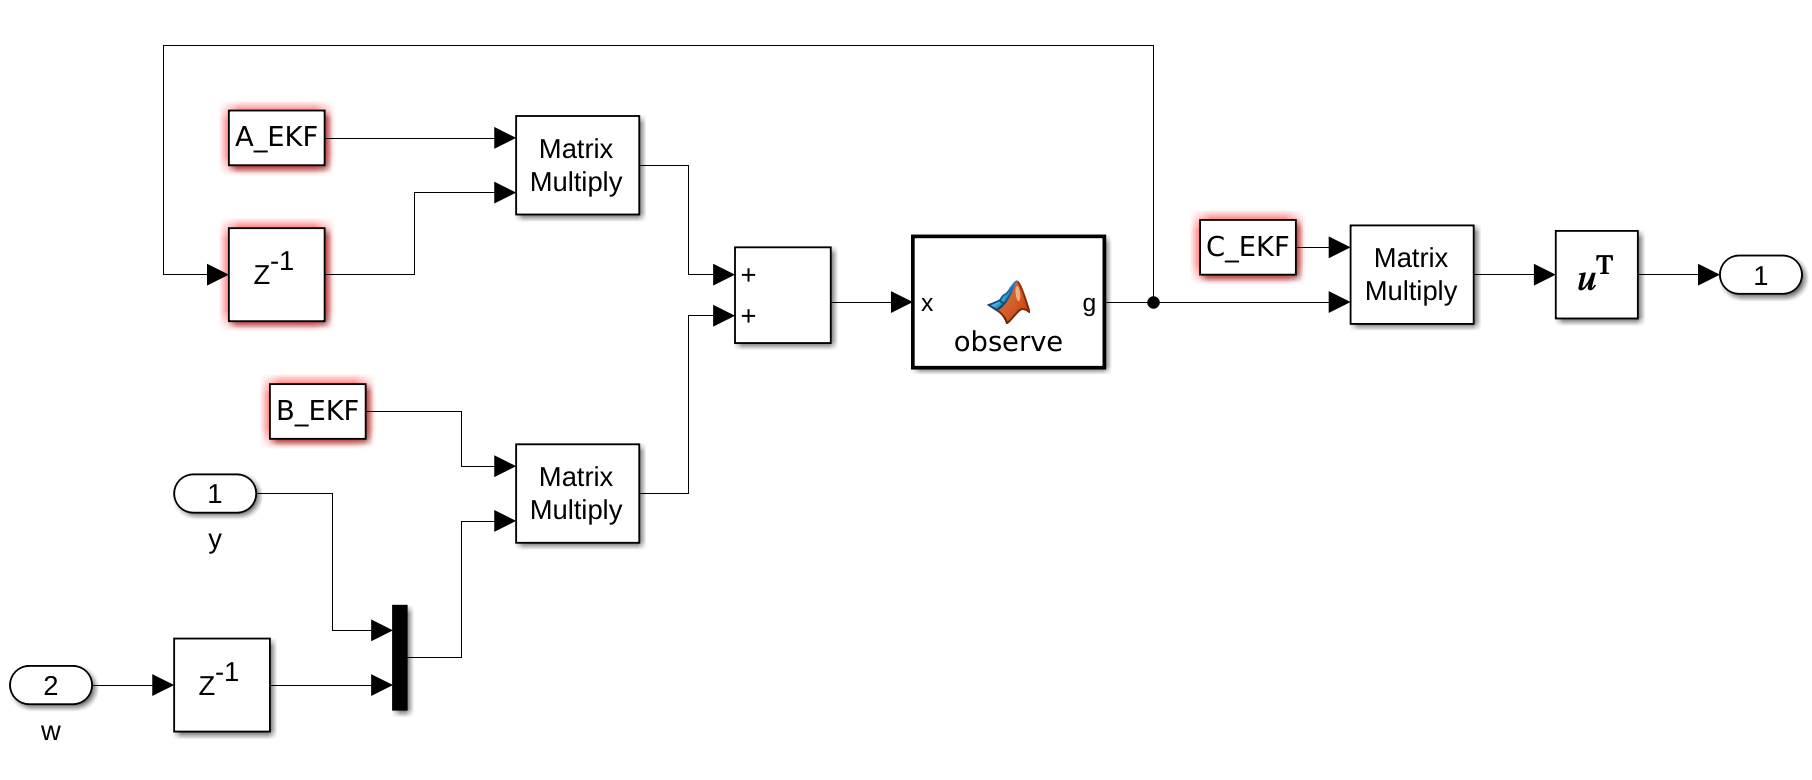
\includegraphics[width=\textwidth]{Figures/Koopman_Block.png}
        \caption{Implementazione del modello}
    \end{figure}
\end{frame}

\begin{frame}{Risultati numerici - Riferimento di passo}
    \begin{table}[]
        \begin{tabular}{|llll|}
        \hline
        \textbf{Observer} & \textbf{Size} & \textbf{NRMSE X\_1} & \textbf{NRMSE X\_2} \\    \hline
        EKF         &   0   &   6.0499  &   0.9370  \\  \hline
        Radial      &   10  &   5.0718   &   0.9171  \\
        Radial      &   20  &   4.8033  &   0.9187  \\
        Radial      &   50  &   5.6129  &   0.9331  \\
        Radial      &   100 &   6.0245  &   0.9379  \\  \hline
        Cov-Radial  &   10  &   5.0854  &   0.9171  \\
        Cov-Radial  &   20  &   4.8117  &   0.9187  \\
        Cov-Radial  &   50  &   5.7038  &   0.9342  \\
        Cov-Radial  &   100 &   5.8595  &   0.9364  \\ \hline
        \end{tabular}
        \end{table}
\end{frame}

\begin{frame}{Risultati grafici - Riferimento di passo}
    \begin{figure}
        \centering
        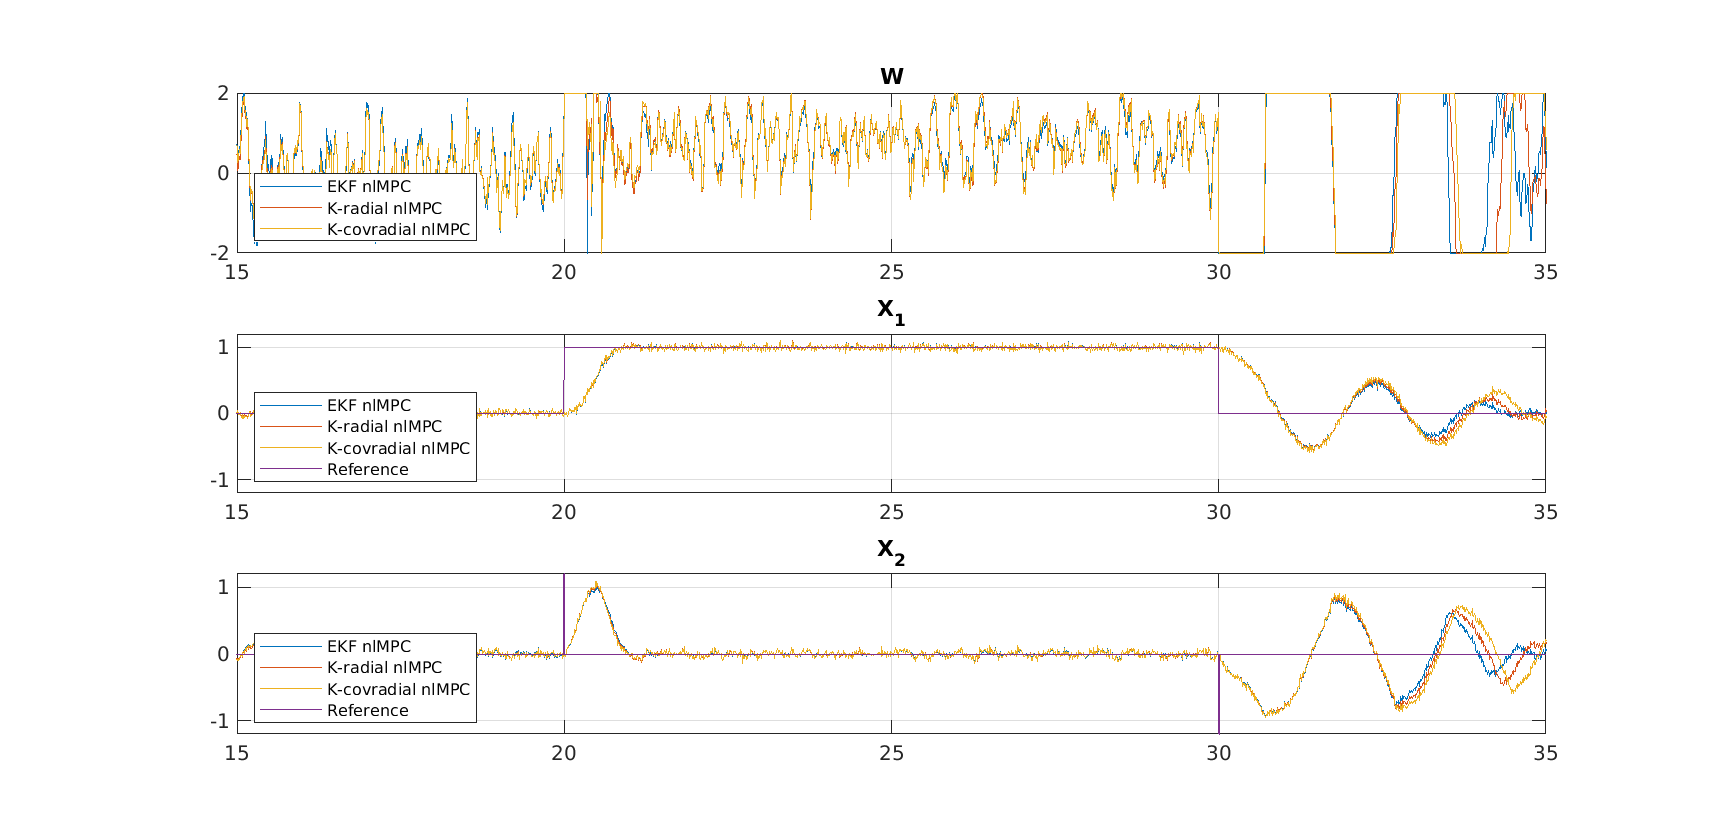
\includegraphics[width=\textwidth]{Figures/step_reference.eps}
    \end{figure}
\end{frame}

\begin{frame}{Risultati numerici - Riferimento oscillante}
    \begin{table}[]
        \begin{tabular}{|llll|}
        \hline
        \textbf{Observer} & \textbf{Size} & \textbf{NRMSE X\_1} & \textbf{NRMSE X\_2} \\    \hline
        EKF         &   0   &   0.3428  &   0.6172  \\  \hline
        Radial      &   10  &   0.3346  &   0.5683  \\
        Radial      &   20  &   0.3318  &   0.5905  \\
        Radial      &   50  &   0.3392  &   0.6048  \\
        Radial      &   100 &   0.3417  &   0.6125  \\  \hline
        Cov-Radial  &   10  &   0.3320  &   0.5645  \\
        Cov-Radial  &   20  &   0.3301  &   0.5872  \\
        Cov-Radial  &   50  &   0.3385  &   0.6051  \\
        Cov-Radial  &   100 &   0.3389  &   0.6078  \\ \hline
        \end{tabular}
        \end{table}
\end{frame}

\begin{frame}{Risultati grafici - Riferimento oscillante}
    \begin{figure}
        \centering
        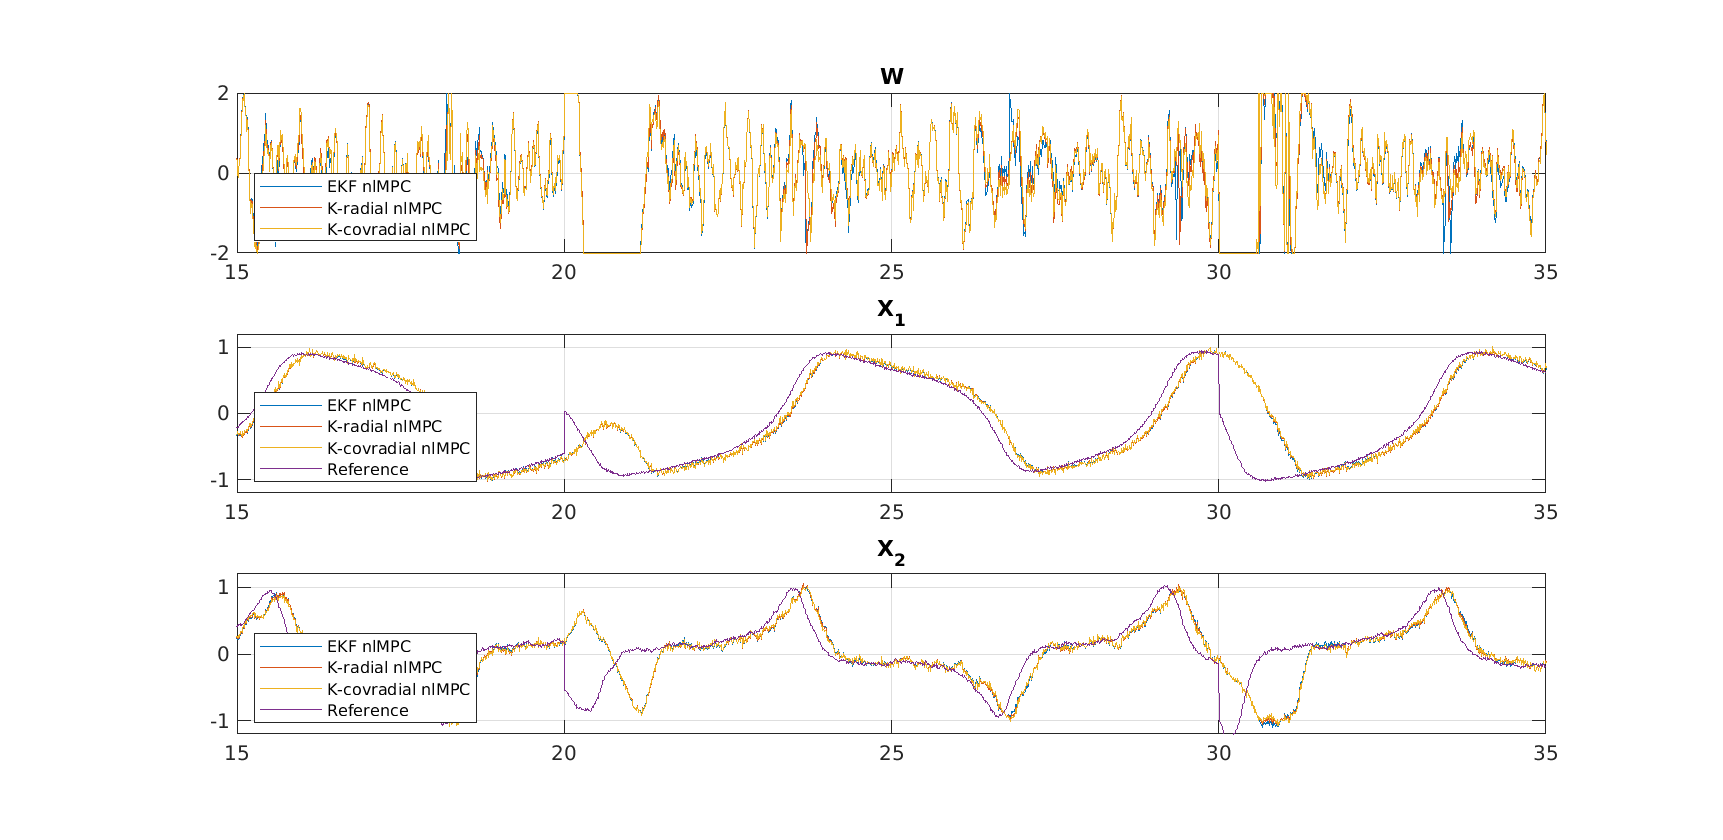
\includegraphics[width=\textwidth]{Figures/osc_reference.eps}
    \end{figure}
\end{frame}

\end{document}